\documentclass[twoside]{book}

% Packages required by doxygen
\usepackage{calc}
\usepackage{doxygen}
\usepackage{graphicx}
\usepackage[utf8]{inputenc}
\usepackage{makeidx}
\usepackage{multicol}
\usepackage{multirow}
\usepackage{textcomp}
\usepackage[table]{xcolor}

% Font selection
\usepackage[T1]{fontenc}
\usepackage{mathptmx}
\usepackage[scaled=.90]{helvet}
\usepackage{courier}
\usepackage{amssymb}
\usepackage{sectsty}
\renewcommand{\familydefault}{\sfdefault}
\allsectionsfont{%
  \fontseries{bc}\selectfont%
  \color{darkgray}%
}
\renewcommand{\DoxyLabelFont}{%
  \fontseries{bc}\selectfont%
  \color{darkgray}%
}

% Page & text layout
\usepackage{geometry}
\geometry{%
  a4paper,%
  top=2.5cm,%
  bottom=2.5cm,%
  left=2.5cm,%
  right=2.5cm%
}
\tolerance=750
\hfuzz=15pt
\hbadness=750
\setlength{\emergencystretch}{15pt}
\setlength{\parindent}{0cm}
\setlength{\parskip}{0.2cm}
\makeatletter
\renewcommand{\paragraph}{%
  \@startsection{paragraph}{4}{0ex}{-1.0ex}{1.0ex}{%
    \normalfont\normalsize\bfseries\SS@parafont%
  }%
}
\renewcommand{\subparagraph}{%
  \@startsection{subparagraph}{5}{0ex}{-1.0ex}{1.0ex}{%
    \normalfont\normalsize\bfseries\SS@subparafont%
  }%
}
\makeatother

% Headers & footers
\usepackage{fancyhdr}
\pagestyle{fancyplain}
\fancyhead[LE]{\fancyplain{}{\bfseries\thepage}}
\fancyhead[CE]{\fancyplain{}{}}
\fancyhead[RE]{\fancyplain{}{\bfseries\leftmark}}
\fancyhead[LO]{\fancyplain{}{\bfseries\rightmark}}
\fancyhead[CO]{\fancyplain{}{}}
\fancyhead[RO]{\fancyplain{}{\bfseries\thepage}}
\fancyfoot[LE]{\fancyplain{}{}}
\fancyfoot[CE]{\fancyplain{}{}}
\fancyfoot[RE]{\fancyplain{}{\bfseries\scriptsize Generated on Tue Oct 31 2017 07\-:58\-:04 for My Project by Doxygen }}
\fancyfoot[LO]{\fancyplain{}{\bfseries\scriptsize Generated on Tue Oct 31 2017 07\-:58\-:04 for My Project by Doxygen }}
\fancyfoot[CO]{\fancyplain{}{}}
\fancyfoot[RO]{\fancyplain{}{}}
\renewcommand{\footrulewidth}{0.4pt}
\renewcommand{\chaptermark}[1]{%
  \markboth{#1}{}%
}
\renewcommand{\sectionmark}[1]{%
  \markright{\thesection\ #1}%
}

% Indices & bibliography
\usepackage{natbib}
\usepackage[titles]{tocloft}
\setcounter{tocdepth}{3}
\setcounter{secnumdepth}{5}
\makeindex

% Hyperlinks (required, but should be loaded last)
\usepackage{ifpdf}
\ifpdf
  \usepackage[pdftex,pagebackref=true]{hyperref}
\else
  \usepackage[ps2pdf,pagebackref=true]{hyperref}
\fi
\hypersetup{%
  colorlinks=true,%
  linkcolor=blue,%
  citecolor=blue,%
  unicode%
}

% Custom commands
\newcommand{\clearemptydoublepage}{%
  \newpage{\pagestyle{empty}\cleardoublepage}%
}


%===== C O N T E N T S =====

\begin{document}

% Titlepage & ToC
\hypersetup{pageanchor=false}
\pagenumbering{roman}
\begin{titlepage}
\vspace*{7cm}
\begin{center}%
{\Large My Project }\\
\vspace*{1cm}
{\large Generated by Doxygen 1.8.6}\\
\vspace*{0.5cm}
{\small Tue Oct 31 2017 07:58:04}\\
\end{center}
\end{titlepage}
\clearemptydoublepage
\tableofcontents
\clearemptydoublepage
\pagenumbering{arabic}
\hypersetup{pageanchor=true}

%--- Begin generated contents ---
\chapter{Hierarchical Index}
\section{Class Hierarchy}
This inheritance list is sorted roughly, but not completely, alphabetically\-:\begin{DoxyCompactList}
\item \contentsline{section}{Neuron}{\pageref{classNeuron}}{}
\begin{DoxyCompactList}
\item \contentsline{section}{Excitatory}{\pageref{classExcitatory}}{}
\item \contentsline{section}{Inhibitory}{\pageref{classInhibitory}}{}
\end{DoxyCompactList}
\item \contentsline{section}{Simulation}{\pageref{classSimulation}}{}
\end{DoxyCompactList}

\chapter{Class Index}
\section{Class List}
Here are the classes, structs, unions and interfaces with brief descriptions\-:\begin{DoxyCompactList}
\item\contentsline{section}{\hyperlink{classExcitatory}{Excitatory} }{\pageref{classExcitatory}}{}
\item\contentsline{section}{\hyperlink{classInhibitory}{Inhibitory} }{\pageref{classInhibitory}}{}
\item\contentsline{section}{\hyperlink{classNeuron}{Neuron} }{\pageref{classNeuron}}{}
\item\contentsline{section}{\hyperlink{classSimulation}{Simulation} }{\pageref{classSimulation}}{}
\end{DoxyCompactList}

\chapter{Class Documentation}
\hypertarget{classExcitatory}{\section{Excitatory Class Reference}
\label{classExcitatory}\index{Excitatory@{Excitatory}}
}
Inheritance diagram for Excitatory\-:\begin{figure}[H]
\begin{center}
\leavevmode
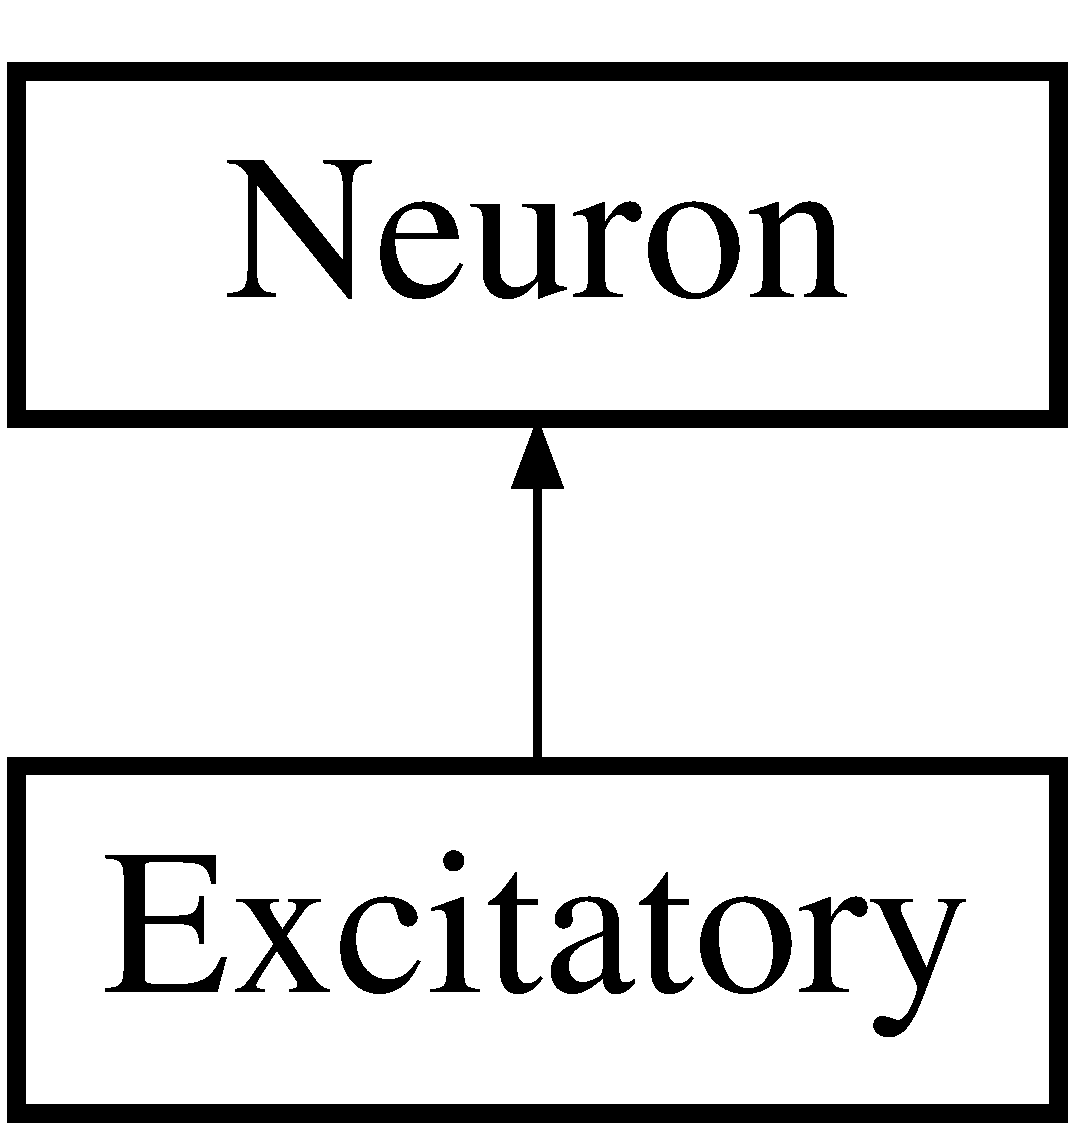
\includegraphics[height=2.000000cm]{classExcitatory}
\end{center}
\end{figure}
\subsection*{Public Member Functions}
\begin{DoxyCompactItemize}
\item 
\hypertarget{classExcitatory_a5512a2acf707cd01901d245282089be6}{{\bfseries Excitatory} (double I\-\_\-ext=I, double Delay=D, double potential=Vr, int local\-\_\-clock=0)}\label{classExcitatory_a5512a2acf707cd01901d245282089be6}

\item 
void \hyperlink{classExcitatory_a62f52a9cc2851b290357d7f4613b9070}{writein\-Buffer} (const int \&time) override
\begin{DoxyCompactList}\small\item\em write in ring buffer. \end{DoxyCompactList}\end{DoxyCompactItemize}
\subsection*{Additional Inherited Members}


\subsection{Member Function Documentation}
\hypertarget{classExcitatory_a62f52a9cc2851b290357d7f4613b9070}{\index{Excitatory@{Excitatory}!writein\-Buffer@{writein\-Buffer}}
\index{writein\-Buffer@{writein\-Buffer}!Excitatory@{Excitatory}}
\subsubsection[{writein\-Buffer}]{\setlength{\rightskip}{0pt plus 5cm}void Excitatory\-::writein\-Buffer (
\begin{DoxyParamCaption}
\item[{const int \&}]{time}
\end{DoxyParamCaption}
)\hspace{0.3cm}{\ttfamily [override]}, {\ttfamily [virtual]}}}\label{classExcitatory_a62f52a9cc2851b290357d7f4613b9070}


write in ring buffer. 

erer 
\begin{DoxyParams}{Parameters}
{\em hallo} & \\
\hline
\end{DoxyParams}
\begin{DoxySeeAlso}{See Also}
hallo 
\end{DoxySeeAlso}
\begin{DoxyReturn}{Returns}
double 
\end{DoxyReturn}


Implements \hyperlink{classNeuron_a41c979859ae91f8f80d58b2d01e1421e}{Neuron}.



The documentation for this class was generated from the following files\-:\begin{DoxyCompactItemize}
\item 
/home/\-I\-N\-T\-R\-A\-N\-E\-T/shmichel/myfiles/3emesemestre/\-Projet/src/Excitatory.\-hpp\item 
/home/\-I\-N\-T\-R\-A\-N\-E\-T/shmichel/myfiles/3emesemestre/\-Projet/src/Excitatory.\-cpp\end{DoxyCompactItemize}

\hypertarget{classInhibitory}{\section{Inhibitory Class Reference}
\label{classInhibitory}\index{Inhibitory@{Inhibitory}}
}
Inheritance diagram for Inhibitory\-:\begin{figure}[H]
\begin{center}
\leavevmode
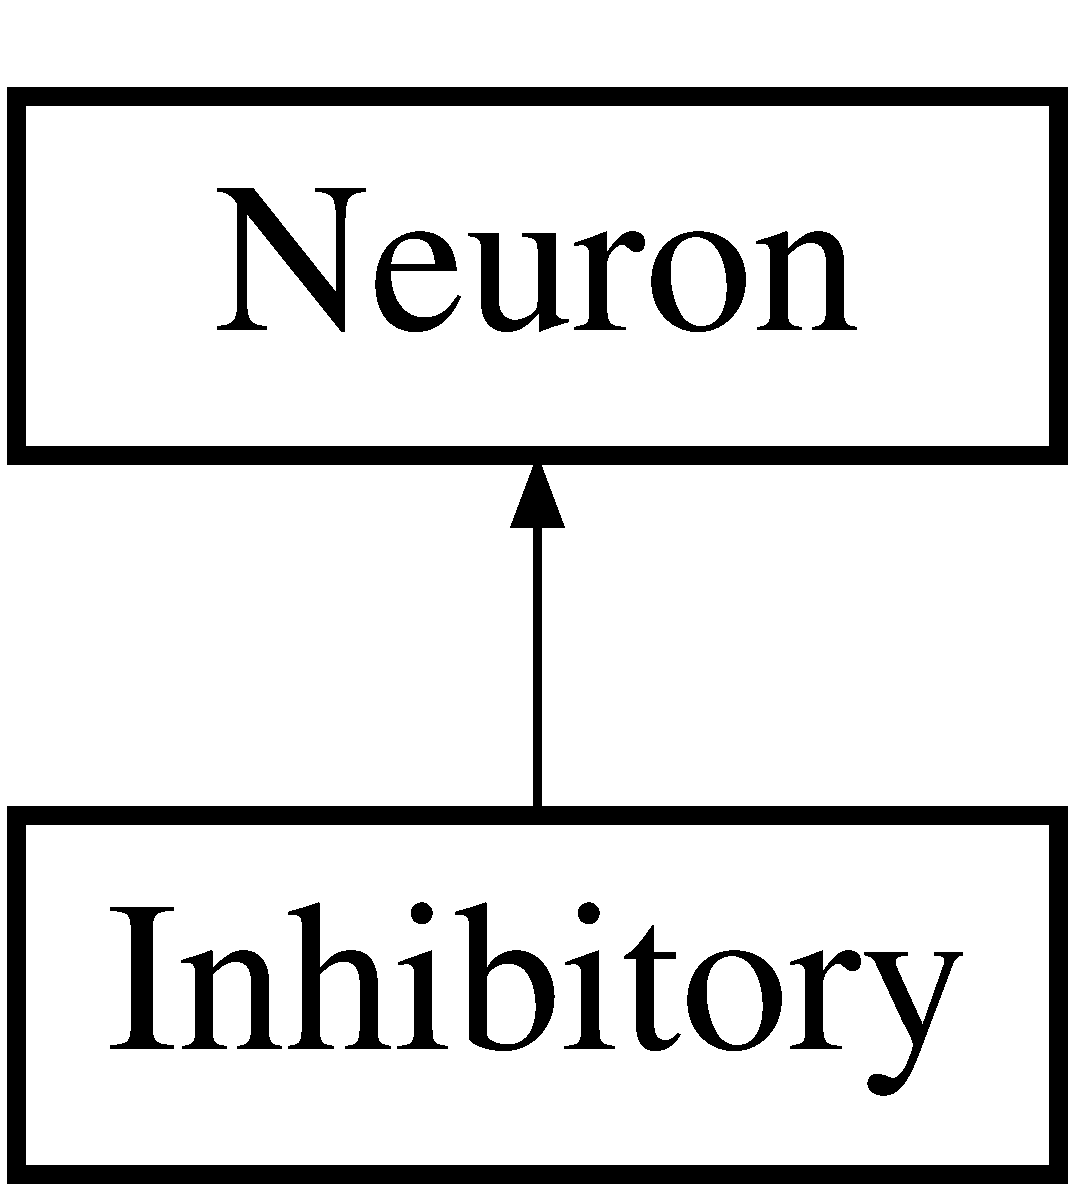
\includegraphics[height=2.000000cm]{classInhibitory}
\end{center}
\end{figure}
\subsection*{Public Member Functions}
\begin{DoxyCompactItemize}
\item 
\hyperlink{classInhibitory_acb4d1d9eaf926ad89a87a110eeda8516}{Inhibitory} (double I\-\_\-ext=I)
\begin{DoxyCompactList}\small\item\em constructor \end{DoxyCompactList}\item 
\hyperlink{classInhibitory_a790c9bdaecdd9fe967caf2833e6eea93}{$\sim$\-Inhibitory} () override
\begin{DoxyCompactList}\small\item\em destructor \end{DoxyCompactList}\item 
void \hyperlink{classInhibitory_a126f7fedd52892995a2017319ee23470}{writein\-Buffer} (const int \&time) override
\begin{DoxyCompactList}\small\item\em writes in its ring buffer the inputs received from spiking neurons it's connected to \end{DoxyCompactList}\end{DoxyCompactItemize}
\subsection*{Additional Inherited Members}


\subsection{Constructor \& Destructor Documentation}
\hypertarget{classInhibitory_acb4d1d9eaf926ad89a87a110eeda8516}{\index{Inhibitory@{Inhibitory}!Inhibitory@{Inhibitory}}
\index{Inhibitory@{Inhibitory}!Inhibitory@{Inhibitory}}
\subsubsection[{Inhibitory}]{\setlength{\rightskip}{0pt plus 5cm}Inhibitory\-::\-Inhibitory (
\begin{DoxyParamCaption}
\item[{double}]{Iexterne = {\ttfamily I}}
\end{DoxyParamCaption}
)}}\label{classInhibitory_acb4d1d9eaf926ad89a87a110eeda8516}


constructor 

Constructor 
\begin{DoxyParams}{Parameters}
{\em external} & current (I as default value) \\
\hline
\end{DoxyParams}
\hypertarget{classInhibitory_a790c9bdaecdd9fe967caf2833e6eea93}{\index{Inhibitory@{Inhibitory}!$\sim$\-Inhibitory@{$\sim$\-Inhibitory}}
\index{$\sim$\-Inhibitory@{$\sim$\-Inhibitory}!Inhibitory@{Inhibitory}}
\subsubsection[{$\sim$\-Inhibitory}]{\setlength{\rightskip}{0pt plus 5cm}Inhibitory\-::$\sim$\-Inhibitory (
\begin{DoxyParamCaption}
{}
\end{DoxyParamCaption}
)\hspace{0.3cm}{\ttfamily [override]}}}\label{classInhibitory_a790c9bdaecdd9fe967caf2833e6eea93}


destructor 

Destructor 

\subsection{Member Function Documentation}
\hypertarget{classInhibitory_a126f7fedd52892995a2017319ee23470}{\index{Inhibitory@{Inhibitory}!writein\-Buffer@{writein\-Buffer}}
\index{writein\-Buffer@{writein\-Buffer}!Inhibitory@{Inhibitory}}
\subsubsection[{writein\-Buffer}]{\setlength{\rightskip}{0pt plus 5cm}void Inhibitory\-::writein\-Buffer (
\begin{DoxyParamCaption}
\item[{const int \&}]{time}
\end{DoxyParamCaption}
)\hspace{0.3cm}{\ttfamily [override]}, {\ttfamily [virtual]}}}\label{classInhibitory_a126f7fedd52892995a2017319ee23470}


writes in its ring buffer the inputs received from spiking neurons it's connected to 

writein\-Buffer S\-U\-B\-S\-T\-R\-A\-C\-T\-S an current at a certain index in the ring buffer for it to be added to the potential latter in the simulation 
\begin{DoxyParams}{Parameters}
{\em time} & at wich the neuron sending the input had a spike \\
\hline
\end{DoxyParams}
\begin{DoxySeeAlso}{See Also}
in \hyperlink{classNeuron_ade349102c17d508352a1061798083ba2}{update} 
\end{DoxySeeAlso}


Implements \hyperlink{classNeuron_a41c979859ae91f8f80d58b2d01e1421e}{Neuron}.



The documentation for this class was generated from the following files\-:\begin{DoxyCompactItemize}
\item 
/home/\-I\-N\-T\-R\-A\-N\-E\-T/shmichel/\-Desktop/myfiles/3emesemestre/\-Projet/src/Inhibitory.\-hpp\item 
/home/\-I\-N\-T\-R\-A\-N\-E\-T/shmichel/\-Desktop/myfiles/3emesemestre/\-Projet/src/Inhibitory.\-cpp\end{DoxyCompactItemize}

\hypertarget{classNeuron}{\section{Neuron Class Reference}
\label{classNeuron}\index{Neuron@{Neuron}}
}
Inheritance diagram for Neuron\-:\begin{figure}[H]
\begin{center}
\leavevmode
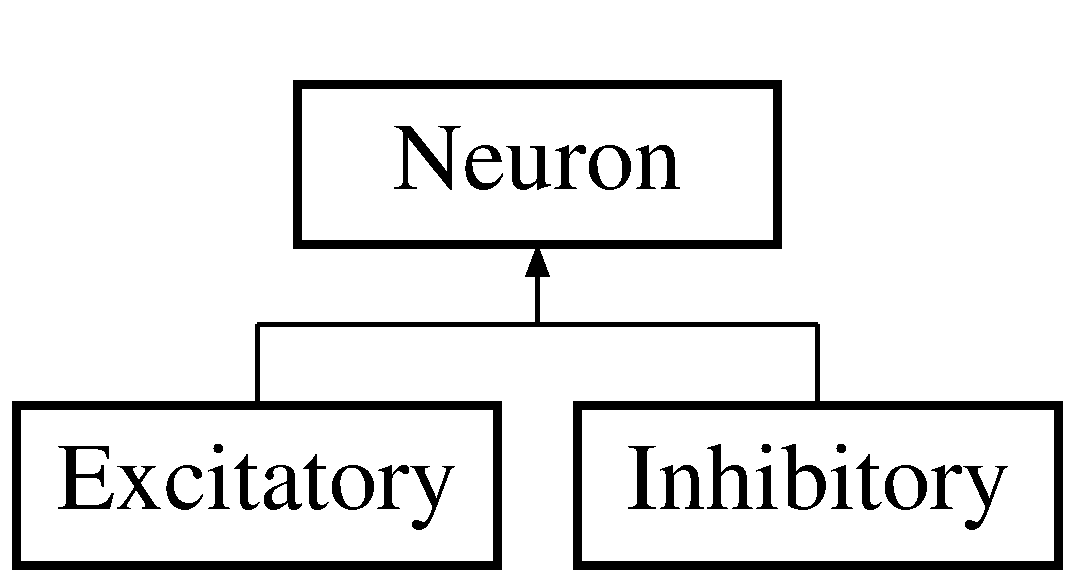
\includegraphics[height=2.000000cm]{classNeuron}
\end{center}
\end{figure}
\subsection*{Public Member Functions}
\begin{DoxyCompactItemize}
\item 
\hyperlink{classNeuron_a7124c9a35644b0ae3fd47f7838c87950}{Neuron} (double I\-\_\-ext, double Delay, double potential, int local\-\_\-clock)
\begin{DoxyCompactList}\small\item\em constructor \end{DoxyCompactList}\item 
\hypertarget{classNeuron_a94a250ce7e167760e593979b899745b1}{virtual \hyperlink{classNeuron_a94a250ce7e167760e593979b899745b1}{$\sim$\-Neuron} ()}\label{classNeuron_a94a250ce7e167760e593979b899745b1}

\begin{DoxyCompactList}\small\item\em destructor \end{DoxyCompactList}\item 
\hypertarget{classNeuron_ae2bc004a58621da0d1c51591400ca87d}{double \hyperlink{classNeuron_ae2bc004a58621da0d1c51591400ca87d}{get\-Potential} () const }\label{classNeuron_ae2bc004a58621da0d1c51591400ca87d}

\begin{DoxyCompactList}\small\item\em gets the potential of the membrane \end{DoxyCompactList}\item 
\hypertarget{classNeuron_af4482bf7c03f6ac6d6a510fd9c022073}{int \hyperlink{classNeuron_af4482bf7c03f6ac6d6a510fd9c022073}{get\-Spike\-Number} () const }\label{classNeuron_af4482bf7c03f6ac6d6a510fd9c022073}

\begin{DoxyCompactList}\small\item\em gets the number of spike since simulation start \end{DoxyCompactList}\item 
\hypertarget{classNeuron_ac800b0047abe17000848648ed81e1017}{int \hyperlink{classNeuron_ac800b0047abe17000848648ed81e1017}{get\-Time\-Spike} () const }\label{classNeuron_ac800b0047abe17000848648ed81e1017}

\begin{DoxyCompactList}\small\item\em gets time of last spike \end{DoxyCompactList}\item 
\hypertarget{classNeuron_a41c979859ae91f8f80d58b2d01e1421e}{virtual void \hyperlink{classNeuron_a41c979859ae91f8f80d58b2d01e1421e}{writein\-Buffer} (const int \&time)=0}\label{classNeuron_a41c979859ae91f8f80d58b2d01e1421e}

\begin{DoxyCompactList}\small\item\em neuron spiking at time (localclock ) sends a signal to every neuron it s connected to \end{DoxyCompactList}\item 
\hypertarget{classNeuron_a7cfb9edb8de019bcaaea6cdf9c8e3b93}{void \hyperlink{classNeuron_a7cfb9edb8de019bcaaea6cdf9c8e3b93}{set\-\_\-\-Iext} (double)}\label{classNeuron_a7cfb9edb8de019bcaaea6cdf9c8e3b93}

\begin{DoxyCompactList}\small\item\em setter of external current \end{DoxyCompactList}\item 
\hypertarget{classNeuron_ade349102c17d508352a1061798083ba2}{bool \hyperlink{classNeuron_ade349102c17d508352a1061798083ba2}{update} ()}\label{classNeuron_ade349102c17d508352a1061798083ba2}

\begin{DoxyCompactList}\small\item\em updates the neuron of one step \end{DoxyCompactList}\end{DoxyCompactItemize}
\subsection*{Protected Attributes}
\begin{DoxyCompactItemize}
\item 
\hypertarget{classNeuron_a772adb0c955d13eb5330560a2bfeafa0}{Buffer {\bfseries buffer\-\_\-}}\label{classNeuron_a772adb0c955d13eb5330560a2bfeafa0}

\end{DoxyCompactItemize}


\subsection{Constructor \& Destructor Documentation}
\hypertarget{classNeuron_a7124c9a35644b0ae3fd47f7838c87950}{\index{Neuron@{Neuron}!Neuron@{Neuron}}
\index{Neuron@{Neuron}!Neuron@{Neuron}}
\subsubsection[{Neuron}]{\setlength{\rightskip}{0pt plus 5cm}Neuron\-::\-Neuron (
\begin{DoxyParamCaption}
\item[{double}]{I\-\_\-ext, }
\item[{double}]{Delay, }
\item[{double}]{potential, }
\item[{int}]{local\-\_\-clock}
\end{DoxyParamCaption}
)}}\label{classNeuron_a7124c9a35644b0ae3fd47f7838c87950}


constructor 

admit initialisation is in ms 

The documentation for this class was generated from the following files\-:\begin{DoxyCompactItemize}
\item 
/home/\-I\-N\-T\-R\-A\-N\-E\-T/shmichel/myfiles/3emesemestre/\-Projet/src/Neuron.\-hpp\item 
/home/\-I\-N\-T\-R\-A\-N\-E\-T/shmichel/myfiles/3emesemestre/\-Projet/src/Neuron.\-cpp\end{DoxyCompactItemize}

\hypertarget{classSimulation}{\section{Simulation Class Reference}
\label{classSimulation}\index{Simulation@{Simulation}}
}
\subsection*{Public Member Functions}
\begin{DoxyCompactItemize}
\item 
\hypertarget{classSimulation_ac8faed6aaf60d10a6b0a6f87c4c90bd2}{\hyperlink{classSimulation_ac8faed6aaf60d10a6b0a6f87c4c90bd2}{Simulation} (int Nb\-Neurones=2)}\label{classSimulation_ac8faed6aaf60d10a6b0a6f87c4c90bd2}

\begin{DoxyCompactList}\small\item\em constuctor \end{DoxyCompactList}\item 
\hypertarget{classSimulation_aa7736d6f953c5e35696b8ac2397a4bea}{void \hyperlink{classSimulation_aa7736d6f953c5e35696b8ac2397a4bea}{Run\-Simulation} ()}\label{classSimulation_aa7736d6f953c5e35696b8ac2397a4bea}

\begin{DoxyCompactList}\small\item\em runs the simulation \end{DoxyCompactList}\item 
void \hyperlink{classSimulation_a2d35287145b4c708ecc473b5ce871ae3}{Update\-Simulation} (int \&global\-Clock)
\begin{DoxyCompactList}\small\item\em updates simulation from global\-Clock until Simulation\-End \end{DoxyCompactList}\item 
void \hyperlink{classSimulation_a59aacc98d8ef86ab6b5b7b1c4f1c92fd}{Create\-Connection} (const size\-\_\-t \&index1, const size\-\_\-t \&index2)
\begin{DoxyCompactList}\small\item\em creates connections between two neurones \end{DoxyCompactList}\item 
\hypertarget{classSimulation_a6fa966b55e89ca6aa6c74f1e9317ee15}{bool {\bfseries Connected} (const size\-\_\-t \&index1, const size\-\_\-t \&index2) const }\label{classSimulation_a6fa966b55e89ca6aa6c74f1e9317ee15}

\item 
\hypertarget{classSimulation_a3fe763c284ff62e74bdf52656251d93a}{unsigned int \hyperlink{classSimulation_a3fe763c284ff62e74bdf52656251d93a}{get\-\_\-\-Nb\-Neurones} () const }\label{classSimulation_a3fe763c284ff62e74bdf52656251d93a}

\begin{DoxyCompactList}\small\item\em return number of neuron in the simulation \end{DoxyCompactList}\item 
\hypertarget{classSimulation_a9bbb7128a50ceb957d6e04f9719b88d1}{double {\bfseries get\-Neurone\-Potential} (size\-\_\-t index) const }\label{classSimulation_a9bbb7128a50ceb957d6e04f9719b88d1}

\end{DoxyCompactItemize}


\subsection{Member Function Documentation}
\hypertarget{classSimulation_a59aacc98d8ef86ab6b5b7b1c4f1c92fd}{\index{Simulation@{Simulation}!Create\-Connection@{Create\-Connection}}
\index{Create\-Connection@{Create\-Connection}!Simulation@{Simulation}}
\subsubsection[{Create\-Connection}]{\setlength{\rightskip}{0pt plus 5cm}void Simulation\-::\-Create\-Connection (
\begin{DoxyParamCaption}
\item[{const size\-\_\-t \&}]{index1, }
\item[{const size\-\_\-t \&}]{index2}
\end{DoxyParamCaption}
)}}\label{classSimulation_a59aacc98d8ef86ab6b5b7b1c4f1c92fd}


creates connections between two neurones 

index1=neurone presynaptique , index2 = neurone postsynaptique

empeche qu un neurone soit connecte a lui meme \hypertarget{classSimulation_a2d35287145b4c708ecc473b5ce871ae3}{\index{Simulation@{Simulation}!Update\-Simulation@{Update\-Simulation}}
\index{Update\-Simulation@{Update\-Simulation}!Simulation@{Simulation}}
\subsubsection[{Update\-Simulation}]{\setlength{\rightskip}{0pt plus 5cm}void Simulation\-::\-Update\-Simulation (
\begin{DoxyParamCaption}
\item[{int \&}]{global\-Clock}
\end{DoxyParamCaption}
)}}\label{classSimulation_a2d35287145b4c708ecc473b5ce871ae3}


updates simulation from global\-Clock until Simulation\-End 

update du neurone dans tous les cas

on rentre dans cette boucle si le neurone a eu un spike variable locale pour optimiser alors pour chaque neurone avec lequel il est connecté, on remplie la case correspondante du buffer 

The documentation for this class was generated from the following files\-:\begin{DoxyCompactItemize}
\item 
/home/\-I\-N\-T\-R\-A\-N\-E\-T/shmichel/myfiles/3emesemestre/\-Projet/src/Simulation.\-hpp\item 
/home/\-I\-N\-T\-R\-A\-N\-E\-T/shmichel/myfiles/3emesemestre/\-Projet/src/Simulation.\-cpp\end{DoxyCompactItemize}

%--- End generated contents ---

% Index
\newpage
\phantomsection
\addcontentsline{toc}{chapter}{Index}
\printindex

\end{document}
